
\chapter{Testowanie aplikacji}

W niniejszym rozdziale przedstawiono proces testowania aplikacji, zarówno w aspekcie manualnym. Testowanie ma na celu weryfikację poprawności działania wszystkich funkcjonalności systemu, sprawdzenie jego stabilności oraz zapewnienie pozytywnych doświadczeń użytkownika.

\section{Testowanie manualne}
Testowanie manualne stanowi kluczowy etap w zapewnieniu jakości aplikacji, zwłaszcza w przypadku interfejsów graficznych (GUI). Polega ono na interakcji z programem z perspektywy końcowego użytkownika, pozwalając na wykrycie problemów z użytecznością, wizualną spójnością oraz błędów, które mogą być trudne do zidentyfikowania za pomocą testów automatycznych. Poniżej przedstawiono wybrane scenariusze testowe, które zostały przeprowadzone manualnie.
\clearpage

\begin{minipage}{\linewidth}
\subsection{Testy scenariuszy logowania i rejestracji}
Kluczowym elementem każdego systemu jest bezpieczne i poprawne zarządzanie kontami użytkowników. Manualne testy tej sekcji obejmowały:
\begin{itemize}
    \item Pomyślne logowanie dla istniejącego użytkownika (klienta detalicznego i administratora).
    \item Logowanie z błędnymi danymi (niepoprawna nazwa użytkownika, niepoprawne hasło).
    \item Testowanie walidacji pól formularza logowania (np. puste pola).
    \item Próba rejestracji użytkownika z istniejącą nazwą użytkownika lub adresem e-mail.
    \item Weryfikacja wyświetlanych komunikatów o błędach. Przykład takiego komunikatu, który informuje o błędnie wprowadzonych danych logowania, widoczny jest na Rysunku \ref{fig:bledne_logowanie}.
\end{itemize}

\begin{figure}[H]
    \centering
    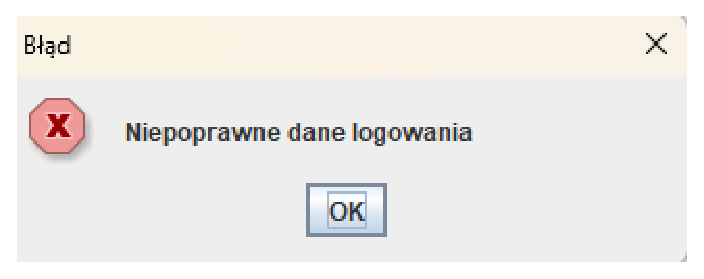
\includegraphics[width=0.5\linewidth]{figures/fig_0004.eps}
    \caption{Komunikat o błędnym wprowadzeniu danych logowania. }
    \label{fig:bledne_logowanie}
    \small{Źródło: Opracowanie własne}
\end{figure}
\end{minipage}

\vspace{1cm}

% --- Blok 2: Opis + Rysunek 4.2 ---
\begin{minipage}{\linewidth}
\subsection{Testy procesu zamawiania dla klienta detalicznego}
Szczególną uwagę zwrócono na poprawność procesu składania zamówienia przez klienta detalicznego. Obejmowało to:
\begin{itemize}
    \item Dodawanie różnych produktów do koszyka i weryfikacja poprawności sumy.
    \item Usuwanie produktów z koszyka i zmiana ich ilości.
    \item Finalizacja zamówienia z poprawnymi danymi klienta (imię, nazwisko, adres, telefon, e-mail).
    \item Testowanie walidacji pól formularza zamówienia (np. puste pola, niepoprawny format e-maila/telefonu). Na Rysunku \ref{fig:bledne_dane_zamowienia} przedstawiono przykład sytuacji, w której dane są niekompletne lub zawierają nieprawidłowe dane, co skutkuje wyświetleniem błędu.
\end{itemize}

\begin{figure}[H]
    \centering
    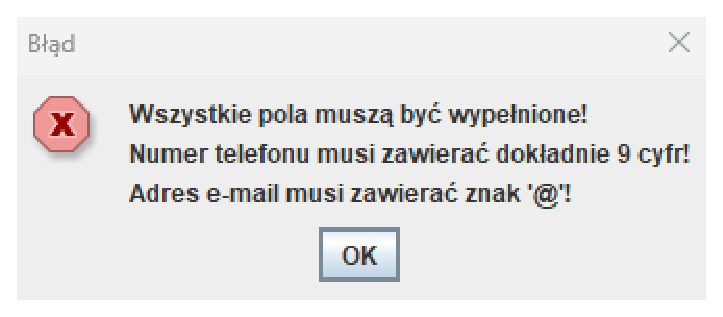
\includegraphics[width=0.5\linewidth]{figures/fig_0005.eps}
    \caption{Przykład błędnego wprowadzenia danych przez klienta detalicznego.}
    \label{fig:bledne_dane_zamowienia}
    \small{Źródło: Opracowanie własne}
\end{figure}
\end{minipage}

\vspace{1cm}


\begin{minipage}{\linewidth}
\subsection{Testy specyficznych scenariuszy klienta hurtowego}
Dla klienta hurtowego przeprowadzono dodatkowe testy, uwzględniające specyfikę jego uprawnień:
\begin{itemize}
    \item Sprawdzenie, czy ceny produktów są wyświetlane jako ceny hurtowe.
    \item Próba złożenia zamówienia z pustym koszykiem. Komunikat informujący o tej sytuacji jest widoczny na Rysunku \ref{fig:pusty_koszyk}.
    \item Testowanie złożenia zamówienia, które nie spełnia minimalnego wymogu dla zamówień hurtowych (jeśli taki istnieje w aplikacji).
    \item Walidacja, czy system odpowiednio reaguje na próby zamówienia zbyt małej ilości produktów.
\end{itemize}

\begin{figure}[H]
    \centering
    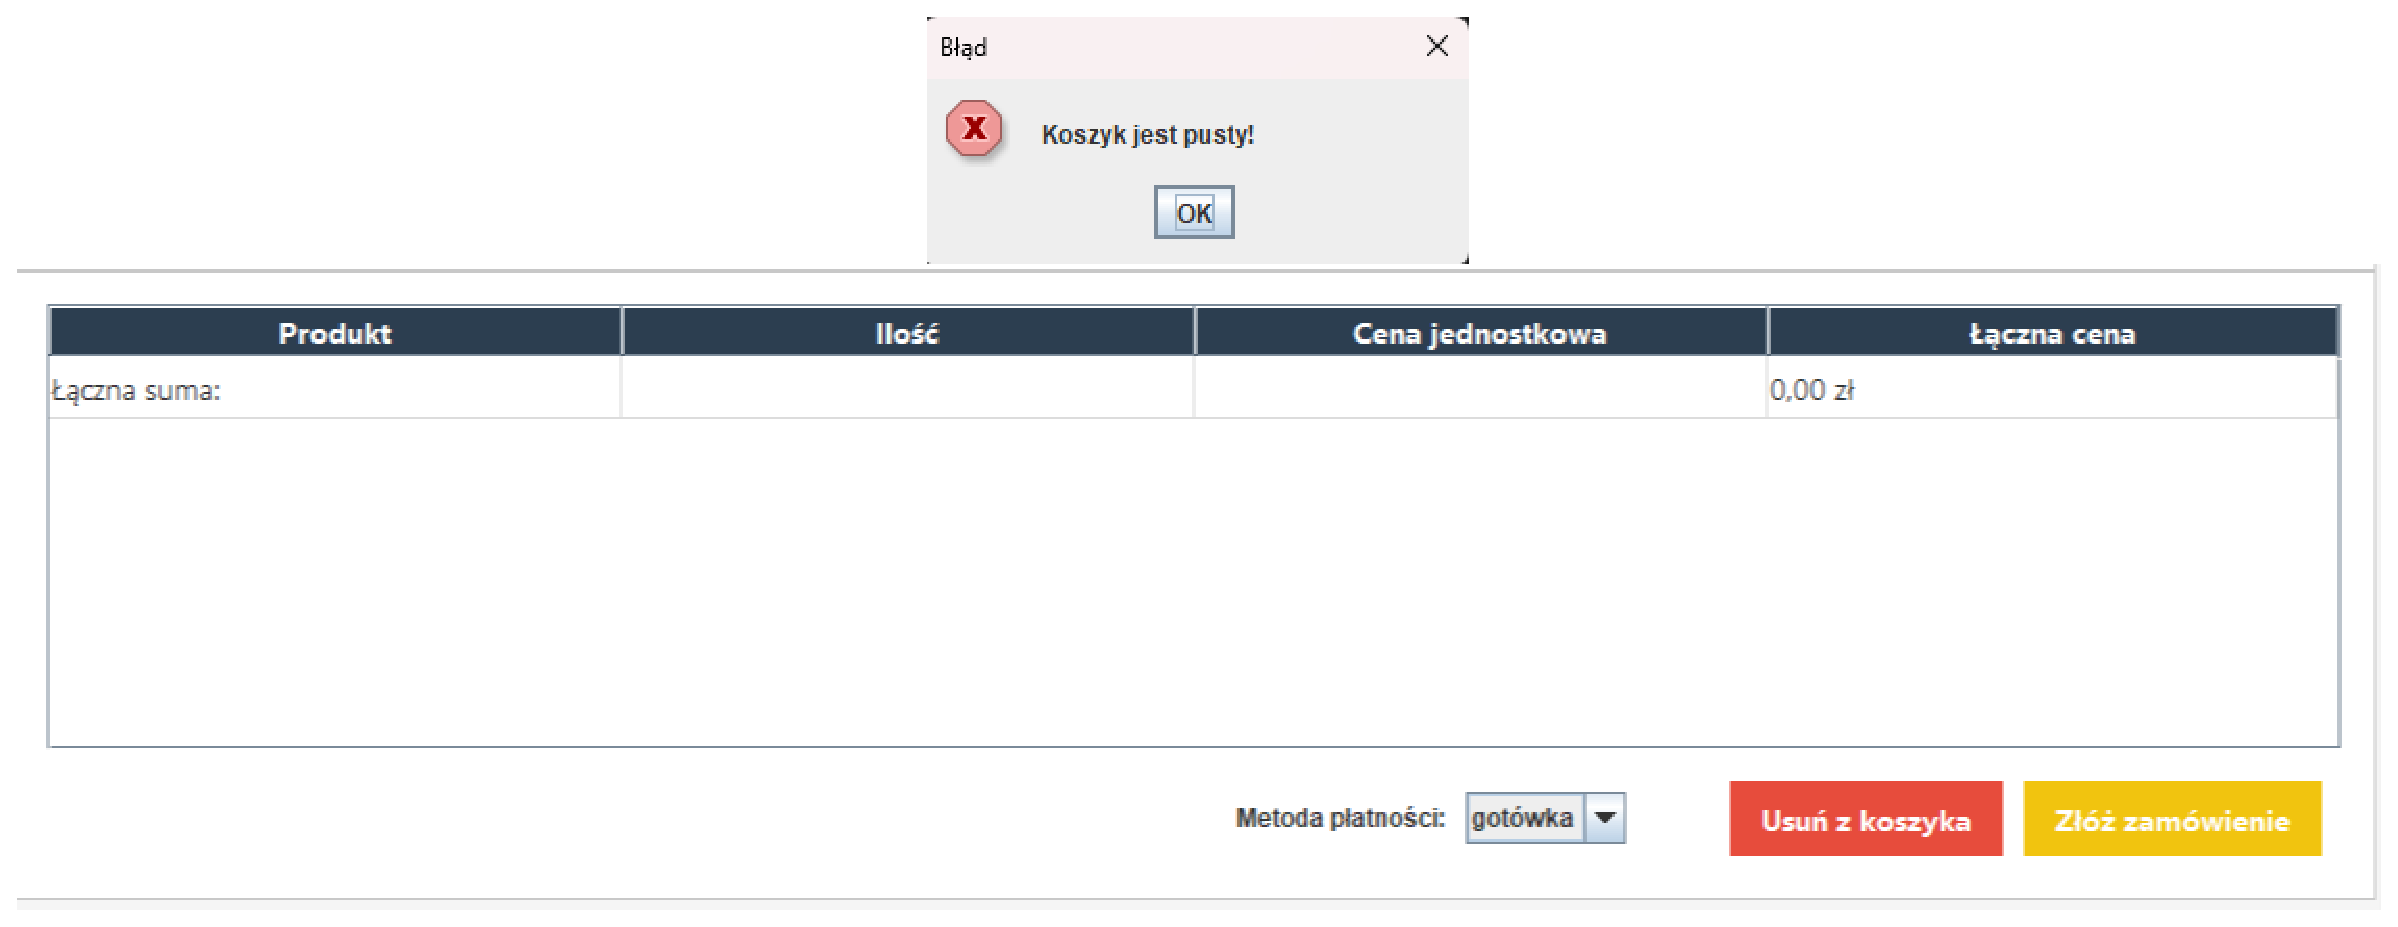
\includegraphics[width=\linewidth]{figures/fig_0006.eps}
    \caption{Komunikat informujący o próbie złożenia zamówienia z pustym koszykiem. }
    \label{fig:pusty_koszyk}
    \small{Źródło: Opracowanie własne}
\end{figure}
\end{minipage}

\subsection{Testy walidacji pól i zabezpieczeń}
W aplikacji zaimplementowano szereg zabezpieczeń i walidacji, które zostały dokładnie przetestowane manualnie. Szczególną uwagę zwrócono na:

\begin{itemize}
    \item Sprawdzenie, czy pola przeznaczone na wartości liczbowe (np. ilość produktów, cena) prawidłowo odrzucają próby wprowadzenia tekstu i akceptują tylko cyfry.
    \item Weryfikację formatu wprowadzanych danych, takich jak adresy e-mail (muszą zawierać znak ‘@’) oraz numery telefonów (muszą składać się z 9 cyfr).
    \item Przetestowanie mechanizmu zmiany hasła, w którym sprawdzono, czy system wymusza identyczność haseł w polach ``nowe hasło'' i ``powtórz nowe hasło''. W przypadku niezgodności, aplikacja wyświetlała odpowiedni komunikat o błędzie.
    \item Dokładne przetestowanie komponentu wyboru daty, LGoodDatePicker \cite{LGoodDatePicker}. Weryfikacja objęła otwieranie i zamykanie kalendarza, wybór daty, ręczne wprowadzanie oraz obsługę błędnych formatów.
    \item Symulację utraty połączenia z bazą danych, aby sprawdzić, czy aplikacja w takiej sytuacji nie ulega awarii, lecz wyświetla użytkownikowi zrozumiały komunikat o problemie.
\end{itemize}